%%%%%%%%%%%%%%%%%%%%%%%%%%%%%%%%%%%%%%%%%
% Beamer Presentation
% LaTeX Template
% Version 1.0 (10/11/12)
%
% This template has been downloaded from:
% http://www.LaTeXTemplates.com
%
% License:
% CC BY-NC-SA 3.0 (http://creativecommons.org/licenses/by-nc-sa/3.0/)
%
%%%%%%%%%%%%%%%%%%%%%%%%%%%%%%%%%%%%%%%%%

%----------------------------------------------------------------------------------------
%	PACKAGES AND THEMES
%----------------------------------------------------------------------------------------

\documentclass{beamer}
\setbeamerfont{institute}{size=\fontsize{7pt}{8pt}}

\mode<presentation> {
	
	% The Beamer class comes with a number of default slide themes
	% which change the colors and layouts of slides. Below this is a list
	% of all the themes, uncomment each in turn to see what they look like.
	
	%\usetheme{default}
	%\usetheme{AnnArbor}
	%\usetheme{Antibes}
	%\usetheme{Bergen}
	%\usetheme{Berkeley}
	%\usetheme{Berlin}
	%\usetheme{Boadilla}
	%\usetheme{CambridgeUS}
	%\usetheme{Copenhagen}
	%\usetheme{Darmstadt}
	%\usetheme{Dresden}
	%\usetheme{Frankfurt}
	%\usetheme{Goettingen}
	%\usetheme{Hannover}
	%\usetheme{Ilmenau}
	%\usetheme{JuanLesPins}
	%\usetheme{Luebeck}
	\usetheme{Madrid}
	%\usetheme{Malmoe}
	%\usetheme{Marburg}
	%\usetheme{Montpellier}
	%\usetheme{PaloAlto}
	%\usetheme{Pittsburgh}
	%\usetheme{Rochester}
	%\usetheme{Singapore}
	%\usetheme{Szeged}
	%\usetheme{Warsaw}
	
	% As well as themes, the Beamer class has a number of color themes
	% for any slide theme. Uncomment each of these in turn to see how it
	% changes the colors of your current slide theme.
	
	%\usecolortheme{albatross}
	\usecolortheme{beaver}
	%\usecolortheme{beetle}
	%\usecolortheme{crane}
	%\usecolortheme{dolphin}
	%\usecolortheme{dove}
	%\usecolortheme{fly}
	%\usecolortheme{lily}
	%\usecolortheme{orchid}
	%\usecolortheme{rose}
	%\usecolortheme{seagull}
	%\usecolortheme{seahorse}
	%\usecolortheme{whale}
	%\usecolortheme{wolverine}
	
	%\setbeamertemplate{footline} % To remove the footer line in all slides uncomment this line
	%\setbeamertemplate{footline}[page number] % To replace the footer line in all slides with a simple slide count uncomment this line
	
	%\setbeamertemplate{navigation symbols}{} % To remove the navigation symbols from the bottom of all slides uncomment this line
}

\usepackage{graphicx} % Allows including images
\usepackage{subfigure}
\usepackage{booktabs} % Allows the use of \toprule, \midrule and \bottomrule in tables
\usepackage{bm}

%----------------------------------------------------------------------------------------
%	TITLE PAGE
%----------------------------------------------------------------------------------------
\useoutertheme{infolines}
\title[Dynamic CMP Neuron]{Dynamic modeling of neural spike count data with non-Poisson variability} % The short title appears at the bottom of every slide, the full title is only on the title page

%\author{Ganchao Wei \textsuperscript{1} \and Ian H. Stevenson \textsuperscript{2, 3}} % Your name

\author[G.\, Wei \& I. H.\, Stevenson]
{%
	\texorpdfstring{
		\begin{columns}%[onlytextwidth]
			\column{.45\linewidth}
			\centering
			Ganchao Wei \textsuperscript{1}\\
			\href{mailto:ganchao.wei@uconn.edu}{ganchao.wei@uconn.edu}
			\column{.45\linewidth}
			\centering
			Ian H. Stevenson \textsuperscript{1, 2}\\
			\href{mailto:ian.stevenson@uconn.edu}{ian.stevenson@uconn.edu}
		\end{columns}
	}
	{Ganchao Wei \& Ian H. Stevenson}
}

\institute[UConn]{
	\textsuperscript{1} Department of Statistics, University of Connecticut   \and
	 \inst{2} Department of Psychological Sciences, University of Connecticut  \and 
	 \inst{3} Department of Biomedical Engineering, University of Connecticut
 }


\date{October 1, 2021} % Date, can be changed to a custom date

\begin{document}
	
	\begin{frame}
		\titlepage % Print the title page as the first slide
	\end{frame}
	
	
	%---------------------------------------------------------
	%	PRESENTATION SLIDES
	%---------------------------------------------------------
	
	\section{Introduction}
	
	\begin{frame}
		\frametitle{Introduction: Neuron and Neural Spikes}
		\textbf{Neuron} and \textbf{Neural Spikes}\\
		Spikes for single neuron: $\{y_k\}_{k=0}^T$ for $y_k \in \mathbb{N}_{\geq 0}$
		\begin{figure}
			\makebox[\linewidth][c]{%
				\centering
				\subfigure[Neuron]{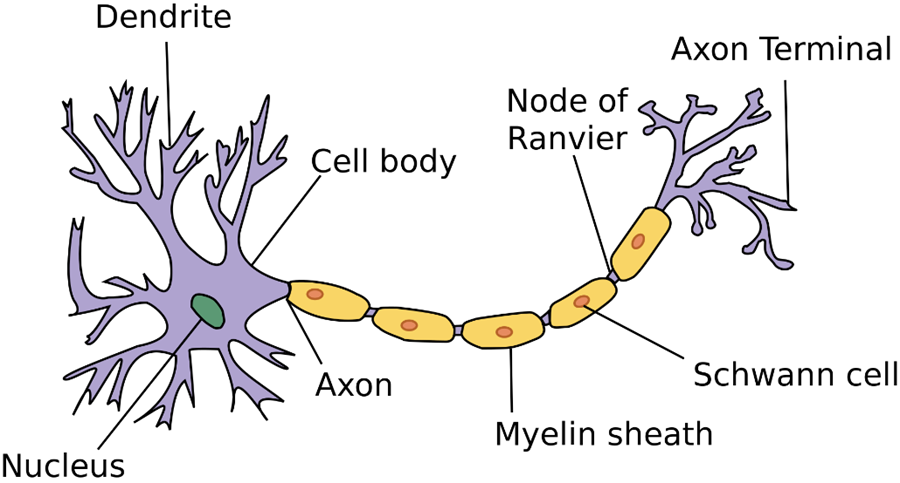
\includegraphics[width=0.4\textwidth]{neuron.png}}%
				\subfigure[Neural Spikes]{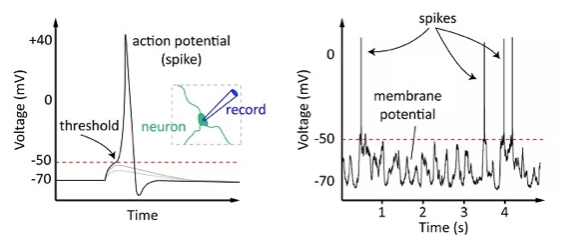
\includegraphics[width=0.4\textwidth]{spike.png}}%
			}
		\end{figure}
		
		Naturally, the spiking pattern (e.g. spiking rate \& variance) will change along the time. \textbf{These changes tell us how brain process information}!
	\end{frame}
	
	%------------------------------------------------
	
	\begin{frame}
		\frametitle{Introduction: Neuron and Neural Spikes}
		Poisson (mean = Var)? NB (mean $\leq$ Var)? \textbf{Unrealistic}!\\
		Fano factor = variance-to-mean ratio $(\sigma^2/ \mu)$
		\begin{figure}
			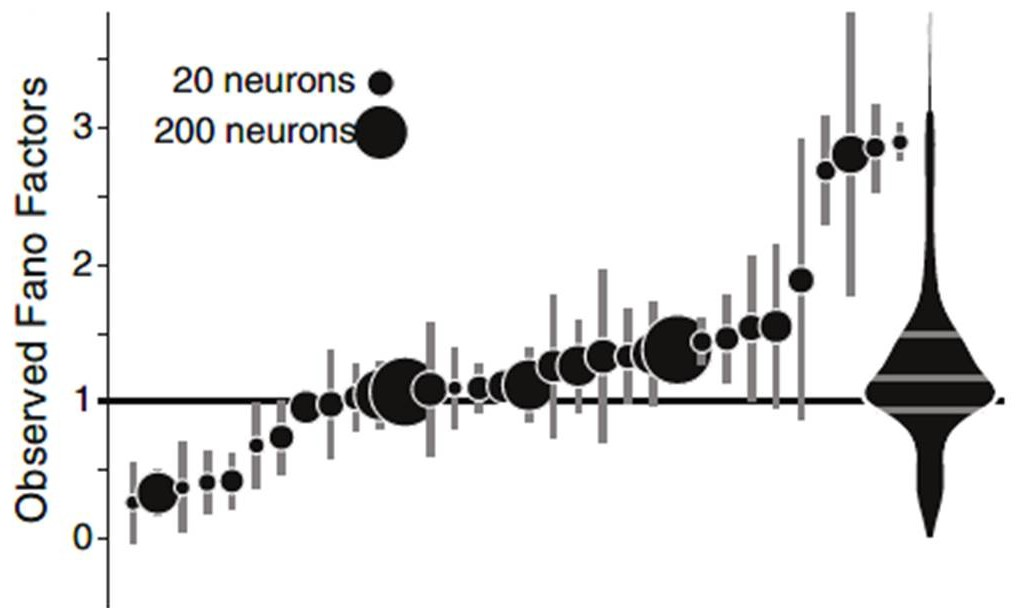
\includegraphics[width=0.5\linewidth]{ff.jpg}
		\end{figure}
		In summary, neural spikes:
		\begin{itemize}
			\item
			pattern (both mean \& variance) changes along the time.
			\item
			non-Poisson, can be both over- and under-dispersed.
		\end{itemize}
	\end{frame}
	
	%------------------------------------------------
	\begin{frame}
		\frametitle{Non-Poisson Counts: Conway-Maxwell Distribution}
		Goal: describe over- and under dispersed count data flexibly.\\
		\textbf{Conway-Maxwell Poisson} (CMP, jointly model \textbf{mean}\& \textbf{variance})\\
		p.m.f. (\(\lambda,\nu > 0\) or
		\(0 < \lambda < 1\), \(\nu = 0\))
		\[P(X = x) = \frac{\lambda^{x}}{(x!)^{\nu}} \cdot \frac{1}{Z(\lambda,\ \nu)}\]
		, for $x = 0, 1,\ldots$ \(Z(\lambda,\nu) = \sum_{y = 0}^{\infty}\frac{\lambda^{y}}{(y!)^{\nu}}\) is the normalizing constant.\\
		Parameter $\nu$ controls the dispersion pattern:
		\begin{itemize}
			\item
			\(\nu = 1\): Poisson
			\item
			\(\nu < 1\): over-dispersed (\(\nu = 0\) Geometric)
			\item
			\(\nu > 1\): under-dispersed (\(\nu \rightarrow \infty\) Bernoulli)
		\end{itemize}
	\end{frame}
	
	%------------------------------------------------
	\begin{frame}
		\frametitle{Track the Change: State Space Model}
		Jointly model parameters of the $i^{th}$ neuron at step $k$: \(\log(\bm{\lambda}_{ik} ) = \bm{X}_{ik}\bm{\beta}_{k}\) and
		\(\log(\bm{\nu}_{ik}) = \bm{G}_{ik}\bm{\gamma}_{k}\). Denote \(\bm{\theta}_{k} = (\bm{\beta}'_{k},\bm{\gamma}'_{k})'\).
		\begin{itemize}
			\item 
			The prior (state equation): $\bm{\theta}_{k}|\bm{\theta}_{k-1}\sim N(\bm{F}_k\bm{\theta}_{k-1}, \bm{Q}_k)$
			\item
			The posterior:
			$P\left( \bm{\theta}_{k} \middle| \bm{Y}_{\lbrack k\rbrack} \right) \propto P\left( \bm{y}_{k} \middle| \bm{\theta}_{k},\ \bm{Y}_{\lbrack k\rbrack} \right)P\left( \bm{\theta}_{k} \middle| \bm{Y}_{\lbrack k - 1\rbrack} \right)$ 
		\end{itemize}
		However, since the likelihood is CMP distributed $\Rightarrow$ no closed posterior.
		Normal approximation: at recursive prior.
		\begin{itemize}
			\item 
			Assume approximated (posterior) gradient \& hessian are the equal to true values.
			\item
			fast: one-time calculation.
		\end{itemize}
	\end{frame}
	
	
	%------------------------------------------------
	\begin{frame}
		\frametitle{Estimation: Filter by Normal Approximation (Original)}
		Normal approximation at recursive prior
		\begin{itemize}
			\item
			Prior:
			\[\bm{\theta}_{k|k - 1} = \bm{F}_{k - 1}\bm{\theta}_{k - 1|k - 1}\]
			\[\bm{\Sigma}_{k|k - 1} = \bm{F}_{k - 1}\bm{\Sigma}_{k - 1|k - 1}\bm{F}'_{k - 1} + \bm{Q}_{k}\]
			\item
			Posterior:
			\[\bm{\theta}_{k|k} = \bm{\theta}_{k|k - 1} + \left( \bm{\Sigma}_{k|k} \right)\left\lbrack \frac{\partial l_{k}}{\partial\bm{\theta}_{k}} \right\rbrack_{\bm{\theta}_{k|k - 1}}\]
			\[\left( \bm{\Sigma}_{k|k} \right)^{- 1} = \left( \bm{\Sigma}_{k|k - 1} \right)^{- 1} - \left\lbrack \frac{\partial^{2}l_{k}}{\partial\bm{\theta}_{k}\partial\bm{\theta}'_{k}} \right\rbrack_{\bm{\theta}_{k|k - 1}}\]
		\end{itemize}
		Great, fast 1-time calculation, but...
		\begin{itemize}
			\item
			Hessian is not robust to outliers.
			\item
			Evaluate things at recursive prior: may bias too much if true values are far from priors.
		\end{itemize}
	\end{frame}
	
	
	%------------------------------------------------
	\begin{frame}
		\frametitle{Improvement}
		\begin{enumerate}
			\item
			Routinely improve filter by backward RTS smoother
			\item
			Ensure positive-definite covariance (robustness): use expected information (like Fisher scoring).
			\item
			Do exact Laplace approximation at the posterior mode: Because of Markovian assumption, the hessian for log-posterior is tri-block diagonal $\Rightarrow$ can update efficiently in $\mathcal{O}(T)$ by Newton-Raphson, starting with smoother estimates.
			\item
			Enlarge the local sample size at each step, by assuming stationary state vectors within a pre-specified window. (select window size by forward-chaining)
		\end{enumerate}
		Both (3) and (4) have their own strengths. When spikes are sparse, (4) is better.
	\end{frame}
	
	%------------------------------------------------
	\begin{frame}
		\frametitle{Simulation}
		\begin{figure}
			\makebox[\linewidth][c]{%
				\centering
				\subfigure[original]{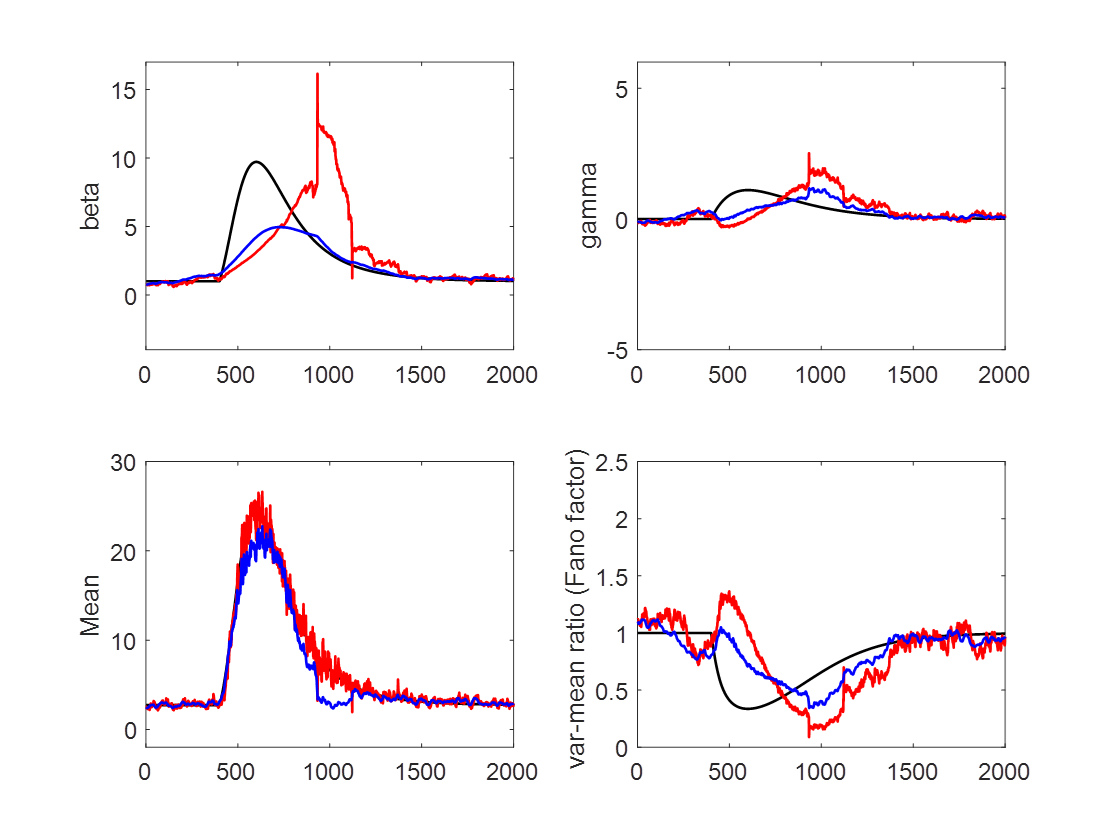
\includegraphics[width=0.5\textwidth]{smoother.png}}%
				\subfigure[after improvement 1, 2 and 4]{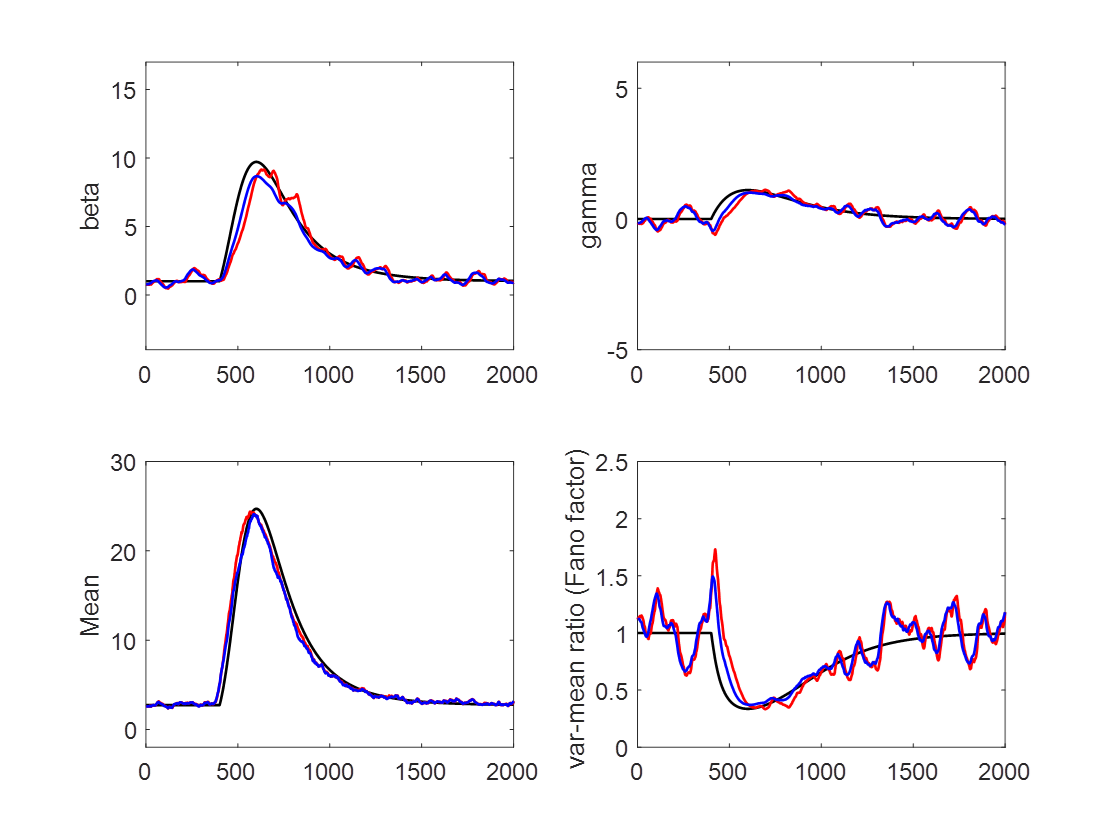
\includegraphics[width=0.5\textwidth]{window.png}}%
			}
		\end{figure}
	\centerline{\textbf{black} = true, \textbf{\textcolor{red}{red}} = filter, \textbf{\textcolor{blue}{blue}} = smoother}
	\end{frame}
	
	%------------------------------------------------
	\begin{frame}
		\frametitle{Application: "place cell" in hippocampus}
		Experiment: a rat run back and forth along the linear track.
		\begin{figure}
			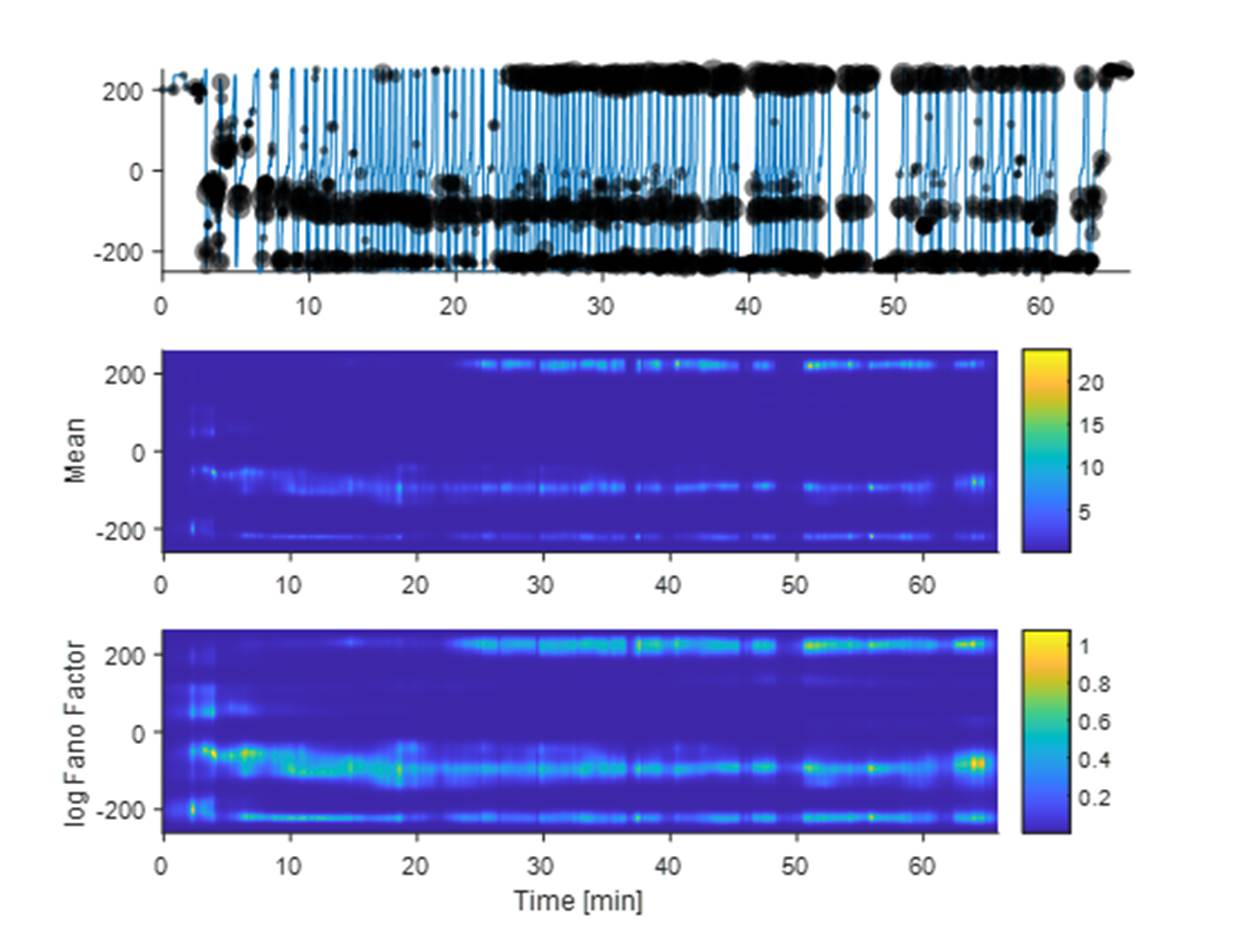
\includegraphics[width=0.7\linewidth]{hippo.jpg}
		\end{figure}
	\end{frame}
	
	%------------------------------------------------
	\begin{frame}
		\frametitle{Appendix 1: Evaluation at Recursive Prior}
		Posterior:
		\begin{align*}
			P(\bm{\theta}_k |\bm{Y}_{[k]}) &\propto L_k\cdot P(\bm{\theta}_k|\bm{Y}_{[k-1]})\\
			&= L_k \cdot \exp\left( - \frac{1}{2}\left( \bm{\theta}_{k} - \bm{\theta}_{k|k - 1} \right)'\left( \bm{\Sigma}_{k|k - 1} \right)^{- 1}\left( \bm{\theta}_{k} - \bm{\theta}_{k|k - 1} \right) \right)\\
			&\propto \exp\left( - \frac{1}{2}\left( \bm{\theta}_{k} - \bm{\theta}_{k|k} \right)'\left( \bm{\Sigma}_{k|k} \right)^{- 1}\left( \bm{\theta}_{k} - \bm{\theta}_{k|k} \right) \right)
		\end{align*}
		Take 1st and 2nd derivatives, w.r.t. $\bm{\theta}_k$:
		\begin{align*}
			\left( \frac{\partial l_{k}}{\partial\bm{\theta}_{k}} \right)^{'} - \left( \bm{\Sigma}_{k|k - 1} \right)^{- 1}\left( \bm{\theta}_{k} - \bm{\theta}_{k|k - 1} \right) &= - \left( \bm{\Sigma}_{k|k} \right)^{- 1}\left( \bm{\theta}_{k} - \bm{\theta}_{k|k} \right)\\
			\frac{\partial^{2}l_{k}}{\partial\bm{\theta}_{k}\partial\bm{\theta}'_{k}} - \left( \bm{\Sigma}_{k|k - 1} \right)^{- 1} &= - \left( \bm{\Sigma}_{k|k} \right)^{- 1}
		\end{align*}
	\end{frame}
	
	%------------------------------------------------
	\begin{frame}
		\frametitle{Appendix 2: Fisher Scoring}
		gradient and hessian of log-likelihood:
		\begin{align*}
			\left\lbrack \frac{\partial l_{k}}{\partial\bm{\theta}_{k}} \right\rbrack_{\bm{\theta}_{k|k - 1}} &= \sum_{i = 1}^{n_{k}}\begin{pmatrix}
				{\left( y_{ik} - E\left( Y_{ik} \right) \right)\bm{x}}_{ik} \\
				{\nu_{ik}\left( E\left( \log{Y_{ik}!} \right) - \log{y_{ik}!} \right)\bm{g}}_{ik} \\
			\end{pmatrix}_{\bm{\theta}_{k|k - 1}}\\
		\left\lbrack - \frac{\partial^{2}l_{k}}{\partial\mathbf{\theta}_{k}\partial\mathbf{\theta}_{k}^{\mathbf{'}}} \right\rbrack_{\mathbf{\theta}_{k|k - 1}} &= \sum_{i = 1}^{n_{k}}\begin{pmatrix}
			A_{ik} & B_{ik}\\
			B'_{ik} & C_{ik}
		\end{pmatrix}
		\end{align*}
		, where
		\begin{align*}
			A_{ik} &= Var(Y_{ik})\bm{x}_{ik}\bm{x}'_{ik}\\
			B_{ik} &= -\nu_{ik}Cov(Y_{ik}, \log Y_{ik}!)\bm{x}_{ik}\bm{g}'_{ik}\\
			C_{ik} &= \nu_{ik}(\nu_{ik}Var(\log Y_{ik}!) - E(\log Y_{ik}!) + \log  y_{ik}!)\bm{g}_{ik}\bm{g}'_{ik}
		\end{align*}
	$C_{ik}$ is not robust to outliers. Replace it by the expected value:	
	$$C_{ik}^* = \nu^2_{ik}Var(\log Y_{ik}!)\bm{g}_{ik}\bm{g}'_{ik}$$
	\end{frame}
	
	%------------------------------------------------
	\begin{frame}
		\frametitle{Appendix 3: Tri-block Diagonal Hessian}
		Hessian for log-posterior:
		\[H = \frac{\partial^{2}\log{P(\bm{\theta}|\mathbf{Y})}}{\partial\bm{\theta}\partial\bm{\theta}^{'}} = \begin{pmatrix}
			\frac{\partial^{2}\log{P(\bm{\theta}|\bm{Y})}}{\partial\bm{\theta}_{1}\partial\bm{\theta}_{1}^{'}} & \bm{F}_{2}^{'}\bm{Q}_{2}^{-1} & \cdots & 0 \\
			\bm{Q}_{2}^{- 1}\bm{F}_{2} & \frac{\partial^{2}\log{P(\bm{\theta}|\bm{Y})}}{\partial\bm{\theta}_{2}\partial\bm{\theta}_{2}^{'}} & \cdots & \vdots \\
			\vdots & \vdots & \ddots & \vdots \\
			0 & \cdots & \cdots & \frac{\partial^{2}\log{P(\bm{\theta}|\bm{Y})}}{\partial\bm{\theta}_{T}\partial\bm{\theta}_{T}^{'}} \\
		\end{pmatrix}\]
		,where
		\begin{align*}
			\frac{\partial^{2}\log{P(\bm{\theta}|\bm{Y})}}{\partial\bm{\theta}_{1}\partial\bm{\theta}_{1}^{'}} &= \frac{\partial^{2}l_{1}}{\partial\bm{\theta}_{1}\partial\bm{\theta}_{1}^{'}} - \bm{\Sigma}_{0}^{- 1} - \bm{F}_{2}^{'}\bm{Q}_{2}^{- 1}\bm{F}_{2}\\
			\frac{\partial^{2}\log{P(\bm{\theta}|\bm{Y})}}{\partial\bm{\theta}_{k}\partial\bm{\theta}_{k}^{'}} &= \frac{\partial^{2}l_{k}}{\partial\bm{\theta}_{k}\partial\bm{\theta}_{k}^{'}} - \bm{Q}_{k}^{- 1} - \bm{F}_{k+1}^{'}\bm{Q}_{k+1}^{- 1}\bm{F}_{k + 1}\\
			\frac{\partial^{2}\log{P(\bm{\theta}|\bm{Y})}}{\partial\bm{\theta}_{T}\partial\bm{\theta}_{T}^{\bm{'}}} &= \frac{\partial^{2}l_{T}}{\partial\bm{\theta}_{T}\partial\bm{\theta}_{T}^{'}} - \bm{Q}_{T}^{- 1}
		\end{align*}
	\end{frame}
	
\end{document}



